% Vložení seznamu příloh
\cleardoublepage
\section*{Seznam příloh}
\label{sec:bla}
\addcontentsline{toc}{section}{Seznam příloh}
\addtocontents{toc}{\protect\setcounter{tocdepth}{-1}}	
\renewcommand\thesection{\appendixname\ \Roman{section}}
\setcounter{section}{0}	
\vspace{-10mm}
% Uprava zobrazeni seznamu příloh kódů
\renewcommand{\cftsecpresnum}{\tablename\enspace+40mm}
\renewcommand{\cftsecaftersnum}{:}
\newlength{\myseclen}
\settowidth{\myseclen}{\cftsecpresnum\cftsecaftersnum}
\addtolength{\cftsecnumwidth}{\myseclen}

\listofappendices\thispagestyle{fancy}
\newpage
\fancyhead[R]{\bfseries\thepage}
\renewcommand{\headrulewidth}{0.5pt}	%tloustka linky v zahlavi
\renewcommand{\footrulewidth}{0pt}		%tloustka linky v zapati
\pagenumbering{Roman}
\renewcommand{\newappendix}[1]{\stepcounter{section}\appendx{#1}}

\newappendix{Grafický návrh uživatelského rozhraní}
	\centering
	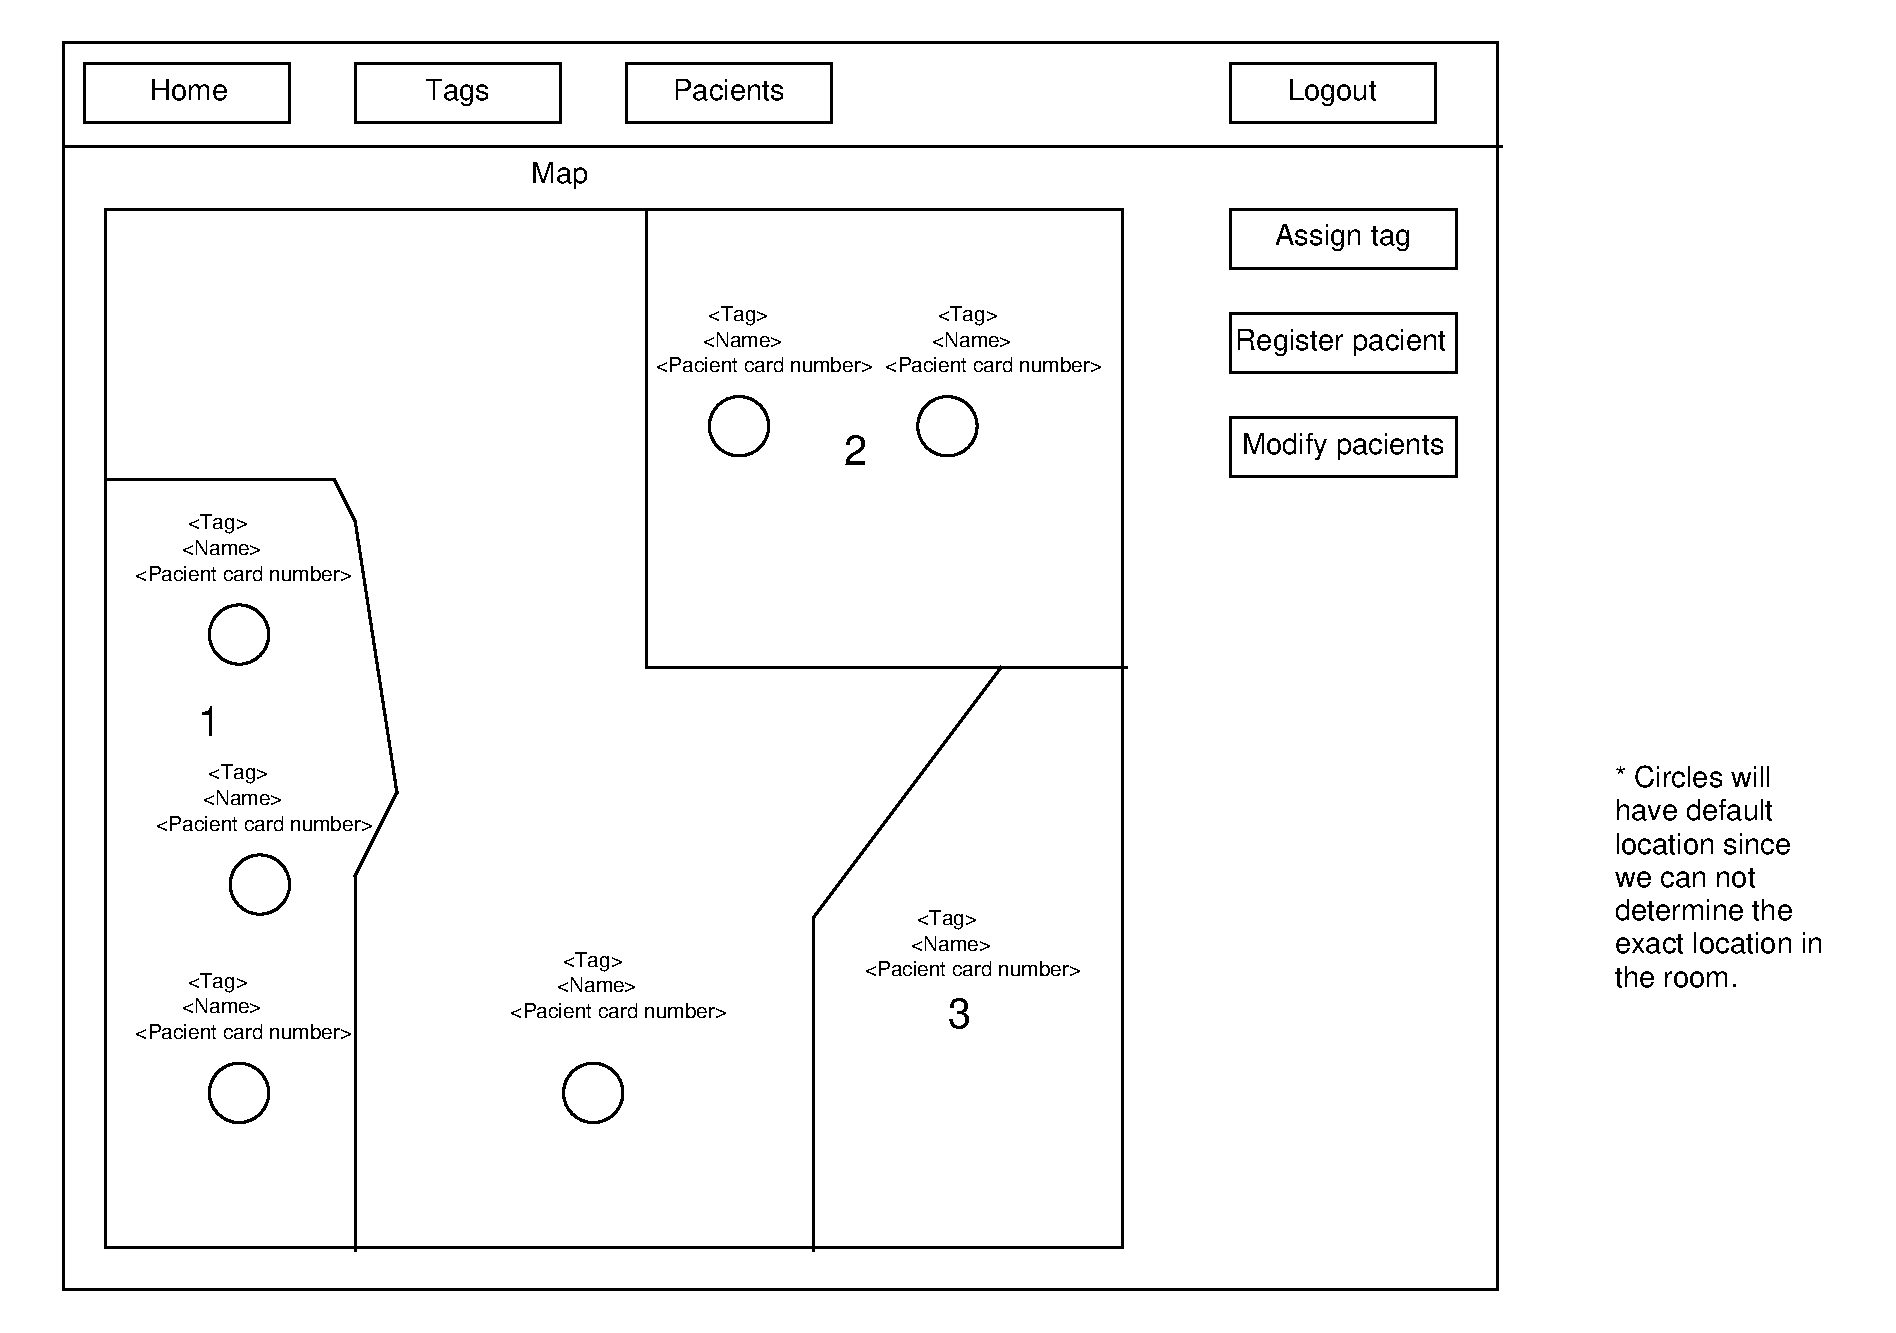
\includegraphics[width=16cm]{Appendix/src/Home.pdf}
	\newline\newline
	Grafický návrh uživatelského rozhraní 1.
	\clearpage
	
\newappendix{Grafický návrh uživatelského rozhraní}
\centering
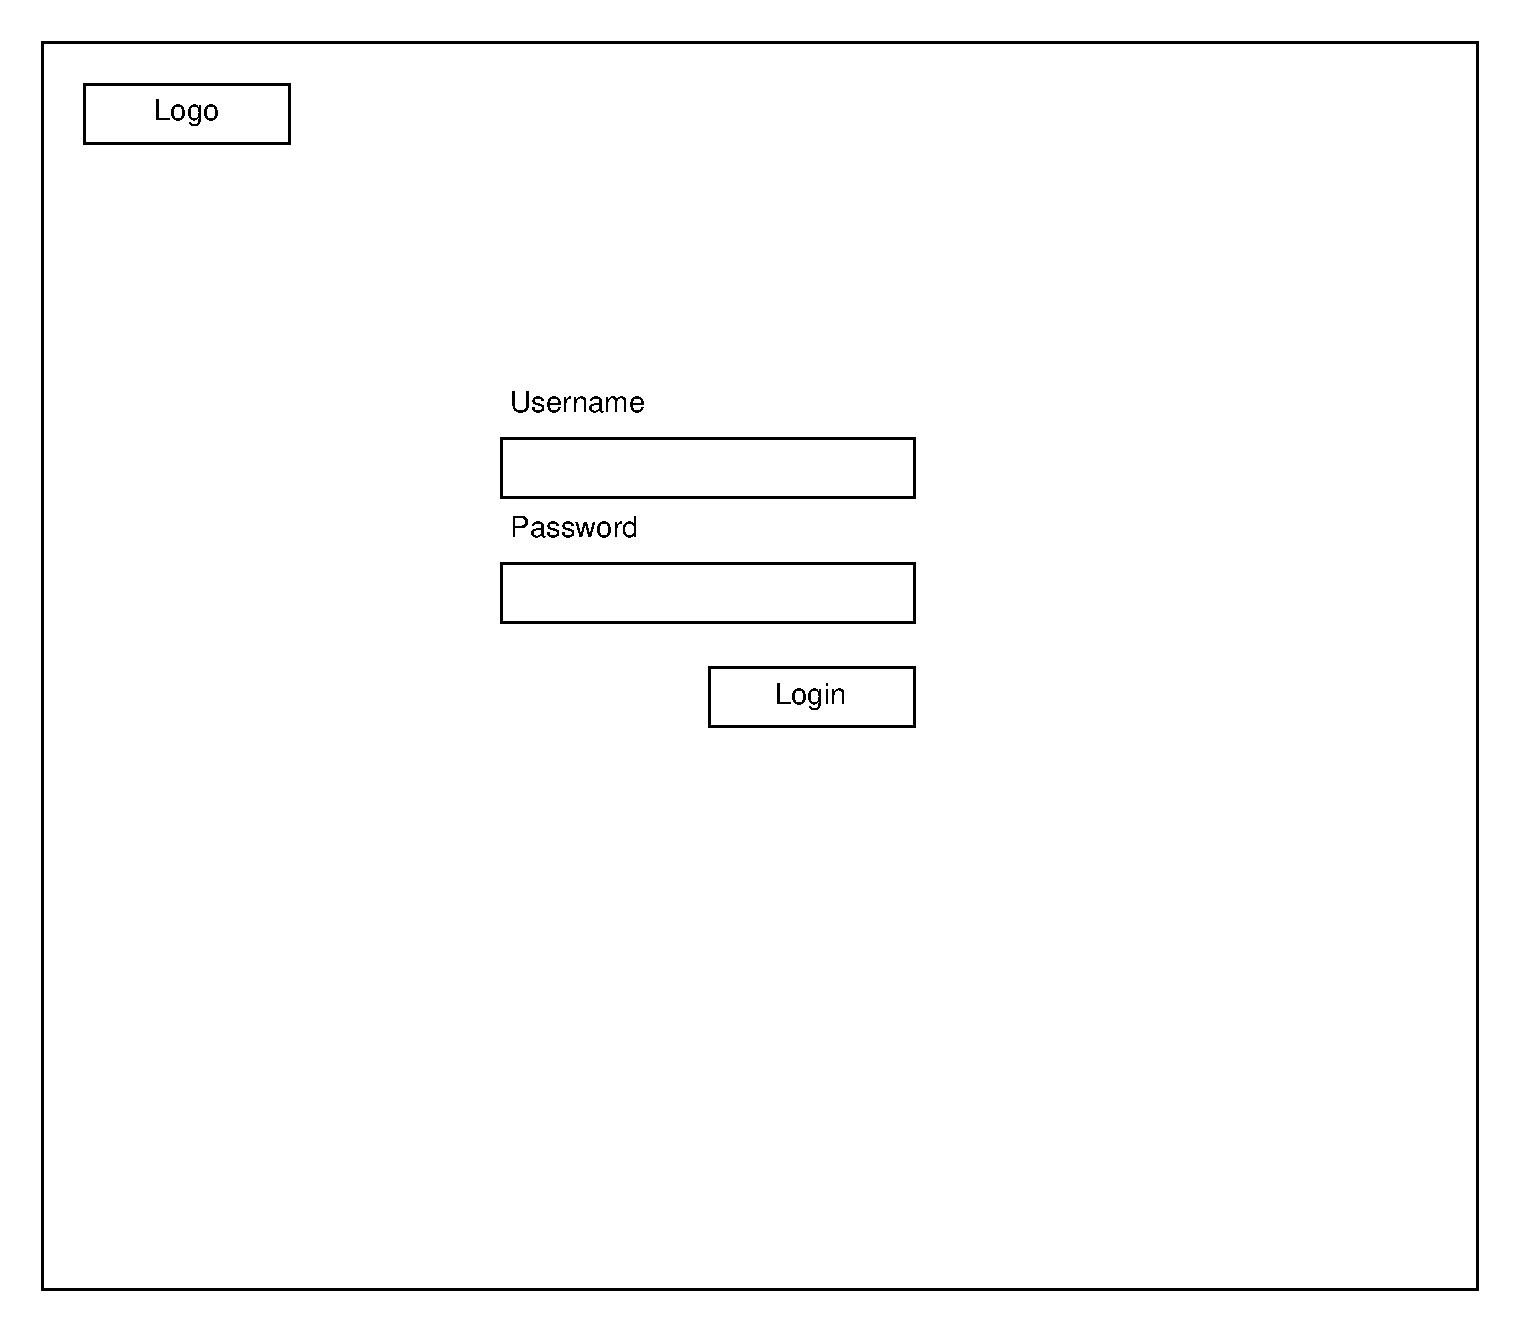
\includegraphics[width=16cm]{Appendix/src/Login.pdf}
\newline\newline
Grafický návrh uživatelského rozhraní 2.
\clearpage


\newappendix{Grafický návrh uživatelského rozhraní}
\centering
\includegraphics[width=16cm]{Appendix/src/Pacients.pdf}
\newline\newline
Grafický návrh uživatelského rozhraní 3.
\clearpage

\newappendix{Grafický návrh uživatelského rozhraní}
\centering
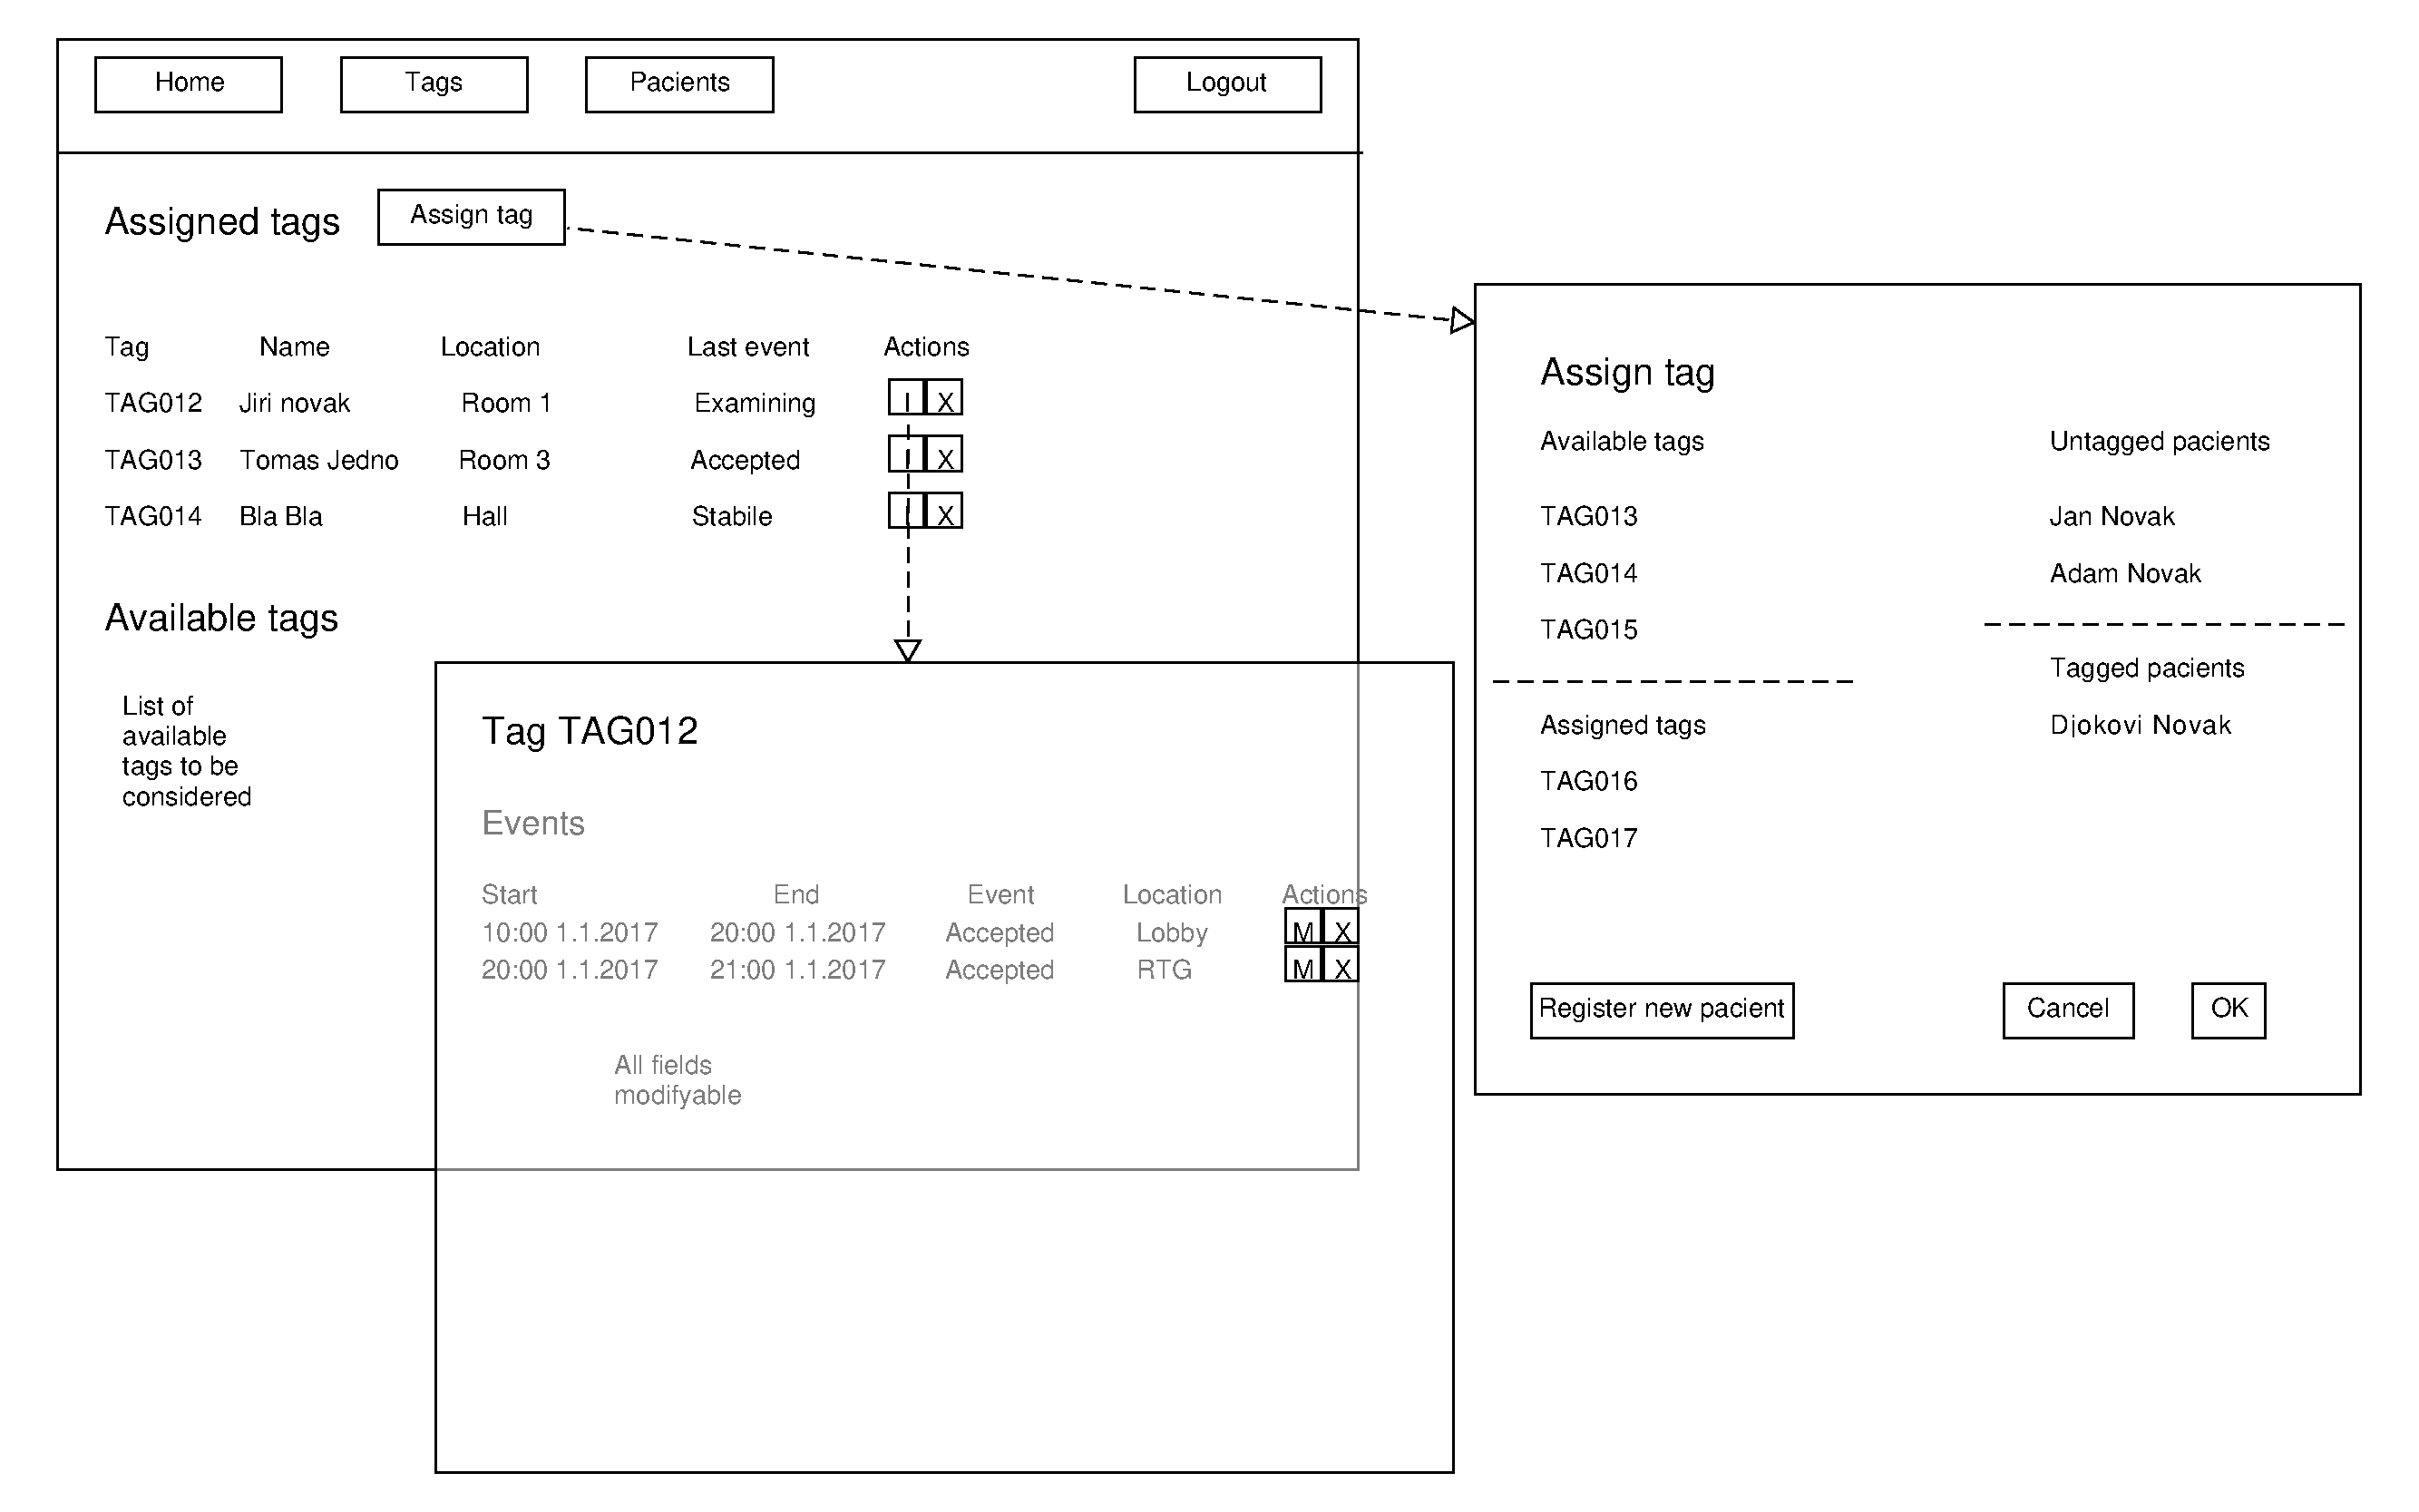
\includegraphics[width=16cm]{Appendix/src/Tags.pdf}
\newline\newline
Grafický návrh uživatelského rozhraní 4.
\clearpage

\newappendix{Přihlašovací okno aplikace}
\centering
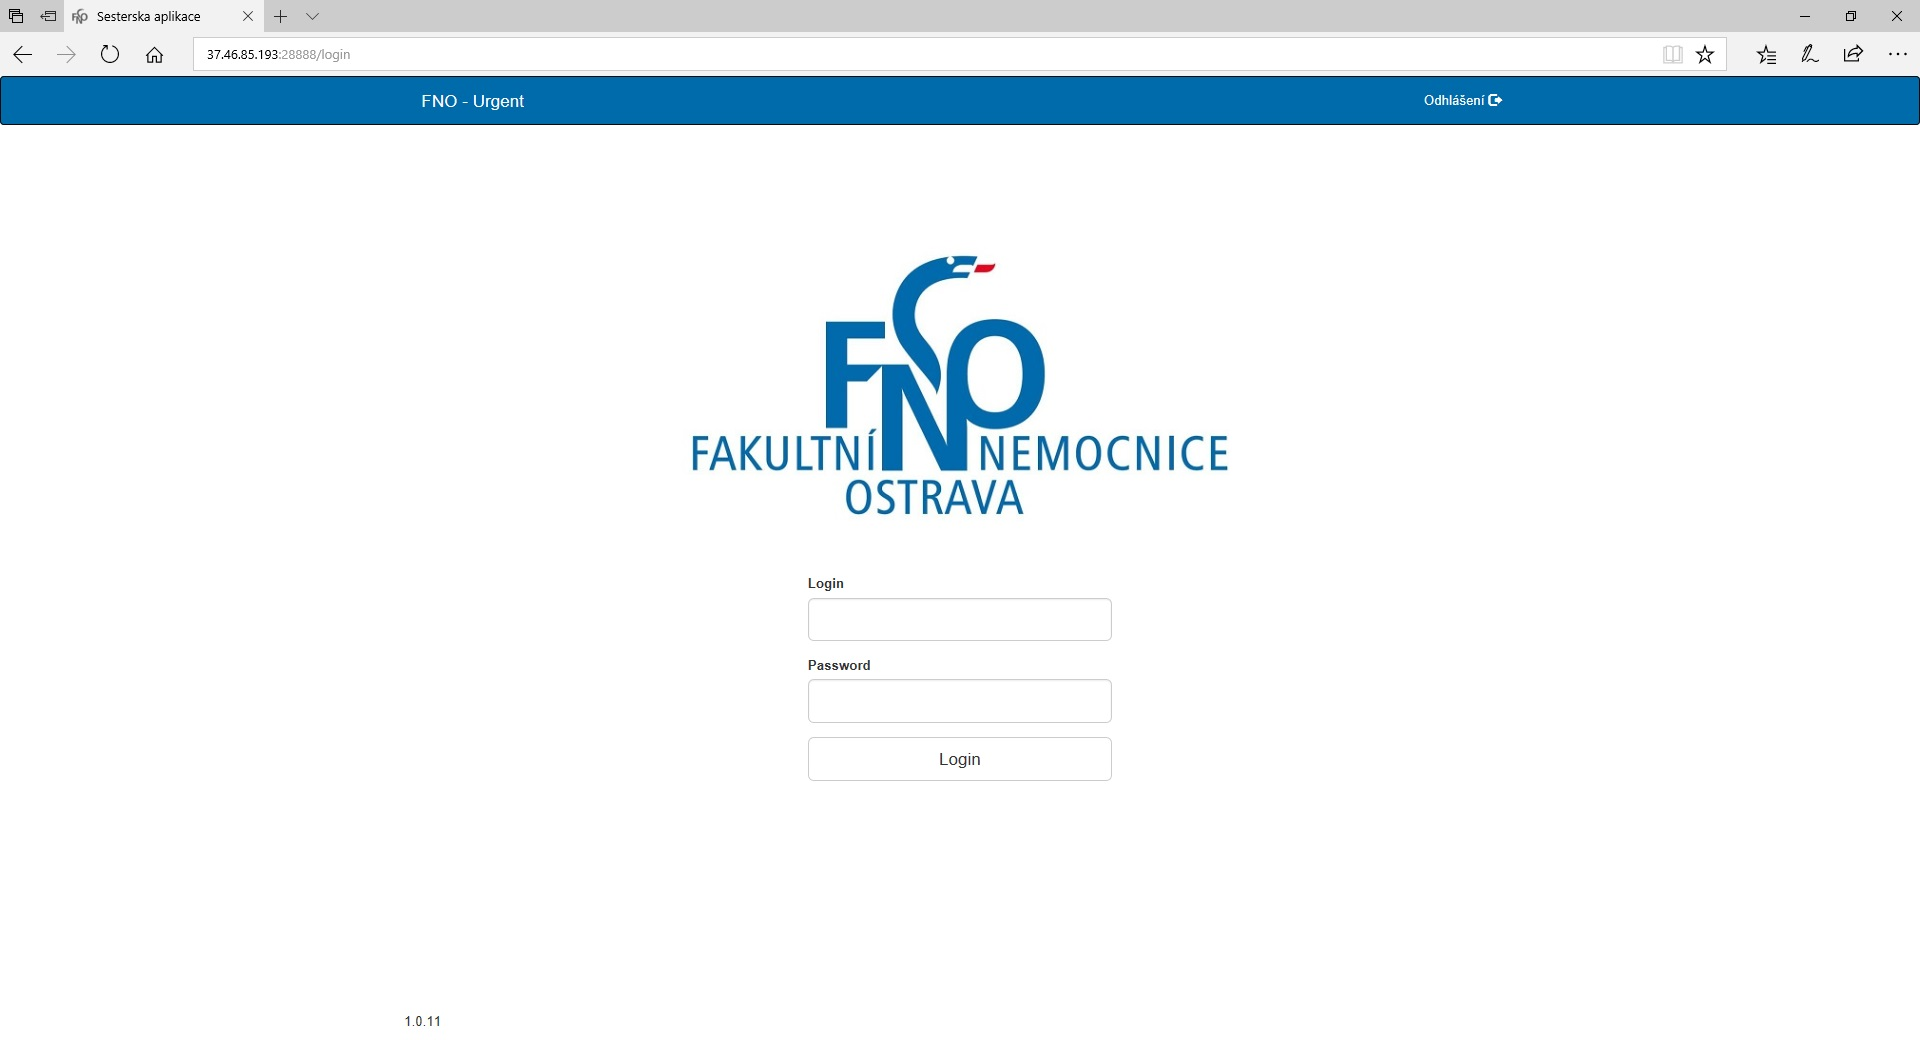
\includegraphics[width=16cm]{Appendix/src/LoginScreen.jpg}
\newline\newline
Přihlašovací okno aplikace.
\clearpage